\chapter{Resultados Experimentais}
\label{cap:resultados}

Para a realização dos testes e coleta dos resultados foram usados dois algoritmos. Um algoritmo para \textbf{Cálculo do Fatorial} (Apêndice~\ref{anexo:fatorial}) e o \textbf{Crivo de Eratóstenes} (Apêndice~\ref{anexo:crivo}).

A escolha do algoritmo fatorial se deve ao fato dessa aplicação já constar como exemplo de aplicações usadas no AppMan. Já o crivo é devido a uma necessidade de maior processamento em relação ao fatorial. 

O Crivo de Eratóstenes é um metodo para encontrar os números primos de um determinado intervalo informado. Ele retira os números múltiplos dos primos menores que a raíz quadrada (arredondada para baixo) do valor máximo no intervalo informado. O exemplo abaixo demonstra a forma de funcionamento do algoritmo:

Suponha que desejamos a lista dos primos entre 1 e 10. Logo $\sqrt{20} \approx 4,47$, então usa-se 4. 

A lista dos números inteiros até o limite: 2, 3, 4, 5, 6, 7, 8, 9, 10, 11, 12, 13, 14, 15, 16, 17, 18, 19, 20. 

O primeiro primo da lista é o número 2. 

Remove-se todos os múltiplos de 2. Ficando como resultado na lista: 2, 3, 5, 7, 9, 11, 13, 15, 17, 19.

O procedimento é repetido para cada primo encontrado na sequência da lista enquando o valor não exceder a 4 que é o limite estipulado na raíz quadrada. Os valores que restarem na lista são os primos para o intervalo estipulado.

Nos testes realizados no AppMan o intervalo estipulado para cálculo foi de 1 até 10000.

O Fatorial é bem mais utilizado, é o produto de todos os inteiros positivos menores ou iguais a um determinado número (n). Na forma matemática descreve-se como \textbf{n!}. O algoritmo utilizado no presente trabalho funciona da seguinte forma:

É definida uma recursiva função que retorna o fatorial do número propriamente dito.

Na programa principal existe um laço que faz o cálculo do fatorial de 8 repetir 10000 vezes acumulando esse resultado.

Ambos algoritmos foram desenvolvidos na linguagem \textbf{C}.

Como já existia o algoritmo fatorial nos arquivos do repositório do AppMan, a realização dos testes com o fatorial ocorreu sem problemas. Já com a aplicação crivo, que foi implementada junto com este trabalho, após submeter as tarefas para o protótipo, este demostrou grande quantidade de erros que impossibilitou a execução. Após uma comparação com o código fonte da aplicação fatorial, notou-se que o programa do crivo esta sem o \emph{status} de saída padrão (\textbf{exit(0)}). Após adicionar a saída padrão do programa crivo o funcionamento com o AppMan ocorreu de forma normal.

A métrica utilizada nos testes foi a escalabilidade. Tentou-se submeter o maior número possível de tarefas em ambas as versões do protótipo. A tabela~\ref{tab:num_max_tarefas} apresenta os números atingidos na submissão das tarefas. No AppMan-RR para a aplicação Fatorial foi possível submeter um número máximo 300 tarefas enquanto que no Crivo o número de tarefas submetidas chegou a 250. Já para AppMan-PBS com a aplicação Fatorial o número de tarefas ficou em 200 e com Crivo foi possível submeter 500 tarefas.

\begin{table}[hbtp]
\begin{center}
\caption{Número Máximo de Tarefas Submetidas}
\label{tab:num_max_tarefas}
\begin{tabular}{c|c|c}
	\hline
		& {\bf AppMan-RR} & {\bf AppMan-PBS}\\
	\hline
	{\bf Crivo} & 250 & 500\\ \hline
	\textbf{Fatorial} & 300 & 200\\ \hline
\end{tabular}
\end{center}
\end{table}

Como dito anteriormente (capitulo~\ref{chap:implementacao}) o AppMan ainda é um protótipo e seu funcionamento nem sempre é o esperado. Foram necessárias algumas tentativas para chegar ao número máximo de tarefas para cada tipo de aplicação. Erros inesperados ocorreram com certa frequência tornando necessário o reinício de toda a submissão. 

Foi possível atingir números além dos transcridos na tabela~\ref{tab:num_max_tarefas}, porém ao analisar os arquivos de saída notou-se que alguns erros foram ocorrido, em alguns casos arquivos necessários para análises não foram gerados completamente. Devido a esse fato essas submissões não foram utilizadas para fins de estatísticas.

\section{Análise do Tempo de Execução das Submissões}

Um dos atributos analisados foi o tempo levado para completar o número de tarefas submetidas. Esse valor é gerado pelo próprio protótipo, ele é iniciado no momento que a aplicação recebe o arquivo \emph{dag}. 

\begin{figure}[htb]
\begin{center}
\includegraphics[scale=0.8]{./img/MapaFatorialTempoTotal.ps}
\caption{Tempo Total \textbf{Fatorial}}
\label{fig:fatorial_total}
Fonte: própria
\end{center}
\end{figure}


asd;fa;sfa;sdfa;sjfa;sjfas;dadfaf

\begin{figure}[htb]
\begin{center}
\includegraphics[scale=0.8]{./img/MapaCrivoTempoTotal.ps}
\caption{Tempo Total \textbf{Crivo}}
\label{fig:crivo_total}
Fonte: própria
\end{center}
\end{figure}
	
